



\documentclass[journal]{IEEEtran}
\hyphenation{op-tical net-works semi-conduc-tor}
%%%%%%%%%%%%%%%%%%%%%%%%%%%%%%%%%%%%%%%%%%%%%%%%%%%%%%%%%%%%%%%%%%
%%%%%%%%%%%%%%%%%%%%%%%%%%%%%%%%%%%%%%%%%%%%%%%%%%%%%%%%%%%%%%%%%%
%%%%%%%%%%%%%%%%%%%%%%%%% PACKAGES %%%%%%%%%%%%%%%%%%%%%%%%%%%%%%%
%%%%%%%%%%%%%%%%%%%%%%%%%%%%%%%%%%%%%%%%%%%%%%%%%%%%%%%%%%%%%%%%%%
%%%%%%%%%%%%%%%%%%%%%%%%%%%%%%%%%%%%%%%%%%%%%%%%%%%%%%%%%%%%%%%%%%
\usepackage[T1]{fontenc}
\usepackage[utf8]{inputenc}
\usepackage{lmodern}
\usepackage[portuguese]{babel}
\usepackage{graphicx}
\usepackage{fancyhdr}
\usepackage{caption}
\usepackage{subcaption}
\usepackage{placeins}
\pagestyle{fancy}
\usepackage{color}
\usepackage{cancel}
\newcommand{\HRule}{\rule{\linewidth}{0.5mm}}
\usepackage{steinmetz}
\graphicspath{{../images/}}
\usepackage{listings}
\lstset{language=C++,
                basicstyle=\ttfamily,
                keywordstyle=\color{blue}\ttfamily,
                stringstyle=\color{red}\ttfamily,
                commentstyle=\color{magenta}\ttfamily,
                morecomment=[l][\color{magenta}]{\#}
}

\begin{document}

\title{
Universidade de Brasília \\
Princípios de Visão Computacional \\
Projeto Final\\
\HRule
\\
Detecção de Objetos \\ {\huge e} \\Previsão de Colisões com 
Filtro de Kalman
\HRule \\
{\normalsize \today}
}

\author{  \begin{tabular}{llr}
    Professor: & Flávio Vidal & \\
    Alunos:& & \\
    & Juarez A.S.F                        & 11/0032829\\
    & Rodrigo Lima 		          & 11/0020090  
      \end{tabular}
      }


\maketitle

%@@@@@@@@@@@@@@@@@@@@@@@@@@@@@@@@@@@@@@@@@@@
%@@@@@@@@@@@@@@@@      OBJETIVOS      @@@@@@
%@@@@@@@@@@@@@@@@@@@@@@@@@@@@@@@@@@@@@@@@@@@
\section{Objetivos}
Desenvolver um algoritmo para detecção de objetos e previsão de
suas trajetórias e possíveis colisões utilizando para isso o 
conjunto de ferramentas disponíveis no OpenCV.
%@@@@@@@@@@@@@@@@@@@@@@@@@@@@@@@@@@@@@@@@@@@@@
%@@@@@@@@@@@@@@        INTRODUÇÃO       @@@@@@
%@@@@@@@@@@@@@@@@@@@@@@@@@@@@@@@@@@@@@@@@@@@@@
\section{Introdução Teórica}
Em aplicações de monitoramento de sistemas móveis estamos muitas vezes
interessados na \textbf{previsão de colisão entre dois objetos}. Com 
essa previsão podemos tomar decisões para evitar a colisão ou, ao 
menos, reduzir os danos causados. Com esse objetivo, \textbf{devemos 
ser capazes detectar os 
objetos}, sua trajetória e sermos capazes de \textbf{extrapolar a 
trajetória e 
prever
as posições futuras} dos objetos sobre monitoramento.

As técnicas de visão computacional são comumente utilizadas na 
detecção de objetos. Vários procedimentos podem ser utilizadas para 
esse fim: como fizemos nos trabalhos anteriores, podemos detectar 
objetos pelo seu contorno(através de gradientes e a transformada 
Canny), sua forma(círculos e retas pela transformada Hough) e pelo 
movimento(subtração de fundo). Nesse trabalho, no entanto, 
usaremos uma técnica mais simples e que é eficiente se conhecermos 
de antemão a cor dos objetos: \textbf{detecção por cor}.


Se as cores dos objetos envolvidos forem conhecidas e aproximadamente 
constantes, e essas cores forem bem distintas das cores do fundo da 
imagem, então basta varremos a imagem procurando os pixeis 
pertencentes a uma certa faixa em torno das cores de interesse e 
temos detectados os objetos.
Uma dificuldade que surge nesse algoritmo, é que cores parecidas podem
ser geradas com combinações diferentes de canais RGB. Para contornar 
esse problema, \textbf{torna-se
útil trabalhar com a imagem em componentes HSV}. HSV é sigla para:
\textbf{REVISAR ESSA DEFINIÇÃO DE HSV!}
\begin{itemize}
 \item 
 \textit{hue}: indica a cor
 \item 
 \textit{saturation}: indica o quanto essa cor está misturado com 
branco
 \item
 \textit{value}: indica o quanto a cor está misturada com preto
\end{itemize}
veja que a componente de cor(\textit{hue}) é obtida diretamente e 
podemos dar maior importância a essa componente na hora da busca.


Utilizando técnicas de transformação morfológicas, como cálculo de 
momentos da imagem, ou então usando o kmeans para agrupar dados 
semelhantes, podemos obter o centro dos objetos sendo detectados e,
monitorando esses centros, guardarmos a trajetória dos objetos a 
medida que o vídeo evolui. Possuindo dados sobre a posição em 
diferentes instantes de tempo podemos \textbf{determinar um modelo} 
envolvendo velocidade e aceleração para calcular uma curva de 
trajetória e assim prever posições futuras para o movimento dos 
objetos.

Esse processo de previsão de uma trajetória pode ser feito utilizando
filtragem de Kalman. \textbf{Filtro de Kalman} é um processo que 
junta informações de um modelo para o sistema sob análise, medições 
realizadas por diferentes sensores e métodos e as incertezas sob o 
modelo e as medições para \textbf{estimar o real valor da variável 
sendo 
medida} e ainda a \textbf{incerteza} resultante dessa estimação.

Podemos
utilizar o filtro de kalman com um modelo de equação do movimento 
envolvendo posição, velocidade e aceleração junto com as medidas 
feitas pelo detector de objetos descrito anteriormente para estimar a 
real posição do objeto. Mas para quê 
utilizarmos o filtro se a detecção por cor já é razoável? Basta 
implementar a detecção para ver o problema: devido a ruídos inerentes
à captura de imagens, é muito provável que, mesmo que o movimento do 
objeto seja suava, \textbf{a detecção perceba uma vibração do centro 
do 
objeto}. Ao utilizarmos o filtro essas vibrações são eliminadas pelo 
modelo e pelo \textbf{conhecimento prévio de um erro gaussiano} nas 
medidas.
Ou seja, \textbf{o filtro não acredita fielmente nas informações dos 
sensores,
ao invés disso, utiliza o modelo para corrigir a detecção}. O quanto 
o filtro acredita nas medidas e no modelo é definido pelo erro 
associado a cada um. Esse erro é, portanto, parte da definição do 
filtro.

Além de estabilizar a detecção, o filtro de Kalman pode ser utilizado 
para \textit{prever o futuro}. Isso é feito ao entrarmos no filtro os 
dados previstos sucessivamente. Isto é, para um conjunto de medidas 
realizada o filtro retorna a posição estimada para o objeto, se 
dissermos para o filtro que essa informação estimada é uma outra 
medida, ele irá processá-la normalmente e retornará a posição 
seguinte. Repetindo o processo, temos uma \textbf{previsão de 
posições 
futuras baseada nos dados medidos e em previsões anteriores do 
filtro}.

Ao fazermos isso teremos uma previsão razoável do futuro dos objetos. 
Falta então procurar por colisões. Para isso \textbf{supomos nossos 
objetos 
como sendo circulares}. O centro da partícula é o centro do objeto 
detectado e para obter o raio podemos usar transformações 
morfológicas e obter o menor círculo que engloba os pixeis 
relacionados a um objeto, ou utilizar o raio do objeto detectado pelo 
kmeans. Para melhorar a previsão, podemos somar ao raio a informação 
de incerteza na posição informada pelo filtro de Kalman. Tendo as 
partículas circulares que englobam os objetos detectados, 
\textbf{basta medir 
a distância entre os dois centros e comparar com a soma dos raios dos 
objetos}. Se a distância for menor que a soma dos raios, então os 
objetos estarão em colisão. Para prever o tempo até a colisão 
dividimos
a distância entre a posição atual a posição prevista de colisão pela
velocidade atual do objeto.



%@@@@@@@@@@@@@@@@@@@@@@@@@@@@@@@@@@@@@@@@@@@
%@@@@@@@@@@@@@@@@      MATERIAIS      @@@@@@
%@@@@@@@@@@@@@@@@@@@@@@@@@@@@@@@@@@@@@@@@@@@

\section{Materiais}
O código elaborado foi feito em C++ com as bibliotecas:
\begin{itemize}
    \item core
    \item imgproc
    \item highgui
    \item background\_segm
    \item tracking
\end{itemize}
do \textbf{OpenCV} versão 2.4.6. Para desenvolver uma interface
visual utilizou-se o Qt versão 5.1.1. e sua IDE Qt Creator para
agilizar o desenvolvimento.
%@@@@@@@@@@@@@@@@@@@@@@@@@@@@@@@@@@@@@@@@@@@
%@@@@@@@@@@@@       PROCEDIMENTOS        @@@
%@@@@@@@@@@@@@@@@@@@@@@@@@@@@@@@@@@@@@@@@@@@
\section{Descrição Experimental}
\begin{itemize}
 \item \textbf{Borrando a Imagem}

    Como é comum em muitos trabalhos de visão computacional,
    os infinitos detalhes e ruídos de uma imagem não são importantes
    para o processamento, de modo que este pode ser otimizado se 
    começarmos por borrar a imagem de entrada. Para isso utilizamos
    um filtro de média dado pela função \textit{medianBlur}. Para
    controlar a intensidade do filtro em templo de execução utilizamos
    um \textit{QComboBox} da biblioteca Qt.
  
  \item \textbf{Detecção de Cor}
 
  Para a detecção de cor utilizamos a rotina \textit{inRange}. Ela 
  recebe a imagem de entrada, um intervalo de cores e cria uma imagem 
  de saída do mesmo tamanho que a de entrada e com branco nos pixeis 
equivalentes da imagem de entrada com cores no intervalo especificado 
e preto no resto. A rotina é chamada para cada cor que se quer 
detectar. Se quisermos detectar n objetos, devemos determinar um 
intervalo para as n cores e teremos ao final n imagens como aquela em
\textbf{REFERÊNCIA AQUI}

\item \textbf{Determinando o Centro dos Objetos}

Para determinar o centro dos objetos, utilizamos a classe 
\textit{Moments}. Essa classe calcula os momentos de uma imagem de 
entrada. O momento de ordem 0 de uma imagem binária nos dá a área
colorida da imagem. Ao dividirmos os momentos de primeira ordem em x 
e em y pelo momento 0 teremos a posição dos centro geométrico da área
pintada na imagem. Se a imagem binária, aquela obtida do procedimento 
anterior, tiver apenas um objeto, o centro calculado será o centro do
objeto sendo detectado(ou ao menos uma boa aproximação dele).

\item \textbf{Filtrando Ruídos}

Para melhorar os resultados dos dois últimos procedimentos filtramos 
a imagem binária antes de determinar o centro dos objetos.
Um filtro de erosão seguido de dilatação diminui pequenas áreas
de ruído e melhorou o processamento. Além disso, pode ser que o objeto
da cor desejada não esteja em cena. Para esses casos adicionamos um 
limiar de threshold para a detecção. Quando a área na imagem binária 
para uma dada cor, dada pelo momento de ordem 0, for menor que um 
determinado limiar indicamos que a detecção falhou e marcamos isso em 
array para posterior referência. Para controle desse limiar em tempo 
de execução, utilizou-se uma trackabr feita de um QSlider e uma 
QLabel, ambos classes da biblioteca Qt.


\item \textbf{Estabilização da Detecção com Filtro de Kalman}

Para estabilizar a detecção utilizou-se o filtro de Kalman 
implementado no OpenCV na classe \textit{KalmanFilter}. Para utilizar
a classe, basta definir as matrizes do filtro e, em cada iteração, 
utilizar o método \textit{predict} seguido do método 
\textit{correct}, onde passamos uma nova medida para \textit{correct}.
A matriz de transição utilizada é mostrada a seguir e implementa um 
modelo com posição, velocidade e aceleração:

\begin{lstlisting}
KF->transitionMatrix =
*(Mat_<float>(6, 6) <<
      /*Sx Sy  Vx Vy Ax   Ay*/
/*Sx*/ 1,  0,  1, 0, 0.5, 0, 
/*Sy*/ 0,  1,  0, 1, 0,   0,
/*Vx*/ 0,  0,  1, 0, 1,   0,
/*Vy*/ 0,  0,  0, 1, 0,   1,
/*Ax*/ 0,  0,  0, 0, 1,   0,
/*Ay*/ 0,  0,  0, 0, 0,   1
);
\end{lstlisting}

e a matriz de medidas:

\begin{lstlisting}
KF->measurementMatrix =
      *(Mat_<float>(2,6) <<
	    1, 0, 1, 0, 0.5, 0,
	    0, 1, 0, 1, 0, 0.5
	);
\end{lstlisting}

\item \textbf{Extrapolando o Movimento com Filtro de Kalman}

Para \textit{prever o futuro} criamos um segundo filtro a partir
de uma cópia do primeiro e repetidamente inserimos nesse novo filtro
suas próprias previsões. Durante o processo as previsões são salvas 
para processamento futuro. Vale ressaltar que cada objeto a ser 
detectado possui seu próprio filtro de estabilização e de previsão do 
futuro, dessa forma temos um vetor de filtros.

\item \textbf{Determinando um Raio}

A definição do 
raio é feita com o auxílio de uma trackbar em tempo de execução.
Para a situação sendo estudada os objetos tem todos mesmos tamanhos, 
dessa forma, em tempo de execução imprimimos os centros das partículas
e, manualmente, setamos um raio adequado para cobrir nossos objetos.
O método foi escolhido por simplicidade de implementação.

\item \textbf{Detectando Colisão}

Varremos os pontos gerados na etapa de previsão e procuramos em quais 
deles, para um mesmo instante de previsão n, tivemos duas partículas
distantes menos que a soma de seus raios individuais. Quando essa
situação ocorrer, marcamos um X preto na tela no ponto médio entre o
centro das duas partículas.

\item \textbf{Controlando o Ambiente}

Dificilmente um algoritmo de visão computacional é robusto à 
iluminação e outras variações do ambiente. Tendo isso em mente, 
um bom sistema baseado em visão costuma ter alguns fatores 
controlados. Desenvolveu-se então uma 'arena' para testes.
Os objetos a serem detectados possuem as cores azul, vermelho e 
amarelo e se locomovem sobre um quadro branco disposto no chão.
A iluminação provém de uma grande e intensa lâmpada colocada 
diretamente a cima do quadro branco.

\end{itemize}

%@@@@@@@@@@@@@@@@@@@@@@@@@@@@@@@@@@@@@@@@@@@@@@@@
%@@@@@@@@@@@@@@@@@@@       DADOS      @@@@@@@@@@@
%@@@@@@@@@@@@@@@@@@@@@@@@@@@@@@@@@@@@@@@@@@@@@@@@
\section{Resultados}

\subsection{Detectando Objetos}
A imagem a seguir mostra a detecção de três objetos de cores 
diferentes. Marcamos com uma cruz o objeto detectado.
\begin{figure}[!htp]
  \centering
  \begin{tabular}{cc}
	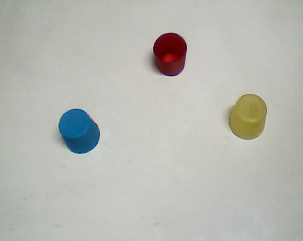
\includegraphics[scale = 0.5]{../images/input.jpg}& 
	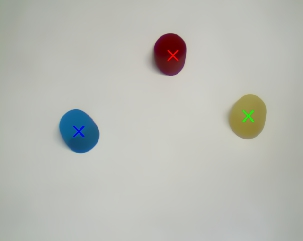
\includegraphics[scale = 0.5]{../images/outputCross.jpg} \\
	{\scriptsize(a)entrada} & {\scriptsize(b)saída} \\
	%	     \multicolumn{2}{c}{\scriptsize(a) }  
  \end{tabular}  
  \caption{detecção de objetos por cor}
  \label{fig:detecSimples}
  \end{figure}
  
\subsection{Kalman para Estabilização}

Nas imagens a seguir vemos o funcionamento do filtro de kalman.
Em \ref{fig:detecSimples}(a) marcamos a detecção por cores com um x e
a detecção com kalman com um círculo. Vemos que com objetos parados 
os dois coincidem. Em \ref{fig:detecSimples}(b) notamos que o 
círculo não acompanha fielmente a cruz: quando o objeto está em 
movimento o círculo está logo atrás do objeto, enquanto a cruz 
continua marcando exatamente.No entanto, quando tampamos o objeto em 
\ref{fig:detecSimples}(c), a cruz se perde, 
enquanto o círculo continua marcando sua posição. Em 
\ref{fig:detecSimples}(d) vemos o filtro estabilizar a detecção. 
Marcamos em azul a trajetória do objeto azul como detectado pelo
algoritmo baseado em cores e em rosa pela algoritmo de Kalman.
Vemos que apesar da trajetória do objeto ter sido oscilante,
a trajetória de Kalman é bem suave.

\begin{figure}[!htp]
  \centering
  \begin{tabular}{cc}
	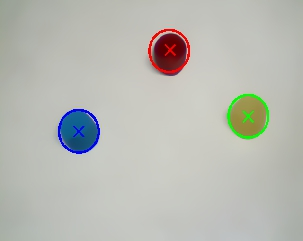
\includegraphics[scale = 0.5]{../images/outputCircle.jpg}& 
	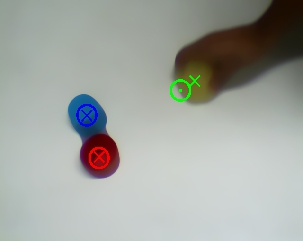
\includegraphics[scale = 0.5]{../images/outoutOnMove.jpg} \\
	{\scriptsize(a)objetos parados} & {\scriptsize(b)objeto em 
movimento} \\
	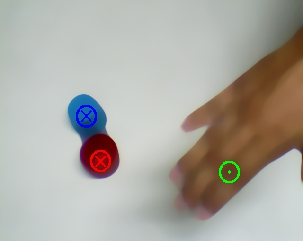
\includegraphics[scale = 
	      0.5]{../images/outputOnHidden.jpg}&
	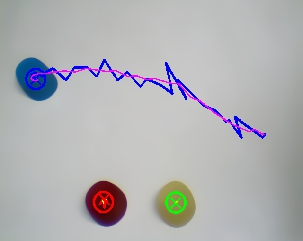
\includegraphics[scale = 
		  0.5]{../images/outputKalmanStable.jpg}\\	
	{\scriptsize(c) objeto escondido}& {\scriptsize(d) 
estabilização da detecção}\\ 
	%\multicolumn{2}{c}{\scriptsize(a) objeto escondido }  
  \end{tabular}  
  \caption{funcionamento do filtro de Kalman}
  \label{fig:KalmanPast}
  \end{figure}

  \subsection{Kalman para Previsão de Colisões}

  Na figure \ref{fig:KalmanFuture} vemos o filtro de Kalman prevendo
  a trajetória futura e prevendo uma colisão. Em 
\ref{fig:KalmanFuture}(a) marcamos com pontos verdes as previsões do 
filtro e em \ref{fig:KalmanFuture}(b) marcamos com um X preto o local
da futura colisão previsto pelo filtro.
  \begin{figure}[!htp]
  \centering
  \begin{tabular}{cc}
	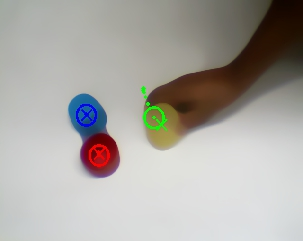
\includegraphics[scale = 0.5]{../images/outputFuture.jpg}& 
	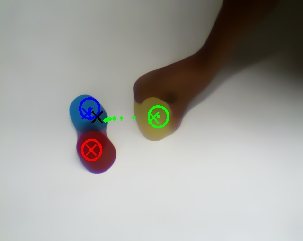
\includegraphics[scale = 0.5]{../images/outputColision.jpg} \\
	{\scriptsize(a)prevendo posições futuras} & 
{\scriptsize(b)prevendo uma colisão} \\
	%\multicolumn{2}{c}{\scriptsize(a) objeto escondido }  
  \end{tabular}  
  \caption{Filtro de Kalman para prever colisões}
  \label{fig:KalmanFuture}
  \end{figure}
%@@@@@@@@@@@@@@@@@@@@@@@@@@@@@@@@@@@@@@@@@@@
%@@@@@@@@@@@@@@       Análise         @@@@@@
%@@@@@@@@@@@@@@@@@@@@@@@@@@@@@@@@@@@@@@@@@@@@
\section{Discussão}


%@@@@@@@@@@@@@@@@@@@@@@@@@@@@@@@@@@@@@@@@@@@@@
%@@@@@@@@@@@@@@       Conclusão         @@@@@@
%@@@@@@@@@@@@@@@@@@@@@@@@@@@@@@@@@@@@@@@@@@@@@

\section{Conclusão}

%@@@@@@@@@@@@@@@@@@@@@@@@@@@@@@@@@@@@@@@@@@@@@@
%@@@@@@@@@@@@@@       REFERÊNCIAS     @@@@@@@@@
%@@@@@@@@@@@@@@@@@@@@@@@@@@@@@@@@@@@@@@@@@@@@@@
\begin{thebibliography}{1}

\bibitem{livroPVC}
Forsyth, D.A. , \emph{Computer Vision: a Modern Approach}, 1ªed.

\bibitem{artigo}
  Vidal, F.B. e Alcalde, V.H.C. \emph{Motion Segmentation in 
Sequential 
  Images Based on the Differential Optical Flow} 

\bibitem{docsOpenCV}
 Documentação do OpenCV
 Disponível em: http://docs.opencv.org
	 Acesso em 21 de Novembro de 2013.

   \bibitem{drawArrows}
    Dan Casas, \emph{how to plot velocity vectors as arrows using
                       sigle static image}.
    Disponível em: 
http://stackoverflow.com/questions/10161351/opencv-how-to-plot-velocit
y-vectors-as-arrows-in-using-single-static-image
    Acesso em 21 de Novembro de 2013.

    \bibitem{kmeans}
    Utkarsh Sinha, \emph{K-Means clustering in OpenCV}.
    Disponível em: 
http://www.aishack.in/2010/08/k-means-clustering-in-opencv/
    Acesso em 21 de Novembro de 2013.

    \bibitem{BGsubtract}
    Mateusz Stankiewicz, \emph{Background detection with OpenCV}.
    Disponível em : http://mateuszstankiewicz.eu/?p=189
    Acesso em 21 de Novembro de 2013. 
\end{thebibliography}

\end{document}


